\section{Method}
\subsection{Producing a Residual Map and Performing Source Detection}
A residual map is produced by modelling the light profiles of the detected sources and subtracting them from the scientific telescope image. Both the COSMOS 2015 and 2020 contain the information necessary to compute a residual map, but differ in their method of performing source extraction and thus also in their method of modelling sources. Since we are interested in objects that are visible in the IRAC bands and not visible in the NIR bands, we aim to produce a residual map of the IRAC image. \\

In the COSMOS 2015 catalogue, the object photometry is carried out using the Source Extraction software  \cite[SExtractor,][]{SExtractor_1996}. To understand how the software works, I performed the source detection using SEP \cite{SEP_2018} (a Python wrapper for SExtractor) on the telescope images from three bands: two optical bands ($g$ and $i$) from HSC\footnote{The Hypersurprime Camera mounted on Subaru} and the near-IR band $Ks$ from VISTA\footnote{The Visible and Infrared Survey Telescope for Astronomy}. The code is available in the notebook \textcolor{darkgray}{Source\_Detection.ipynb} in the linked repository. \textcolor{red}{Should I even reference to the code like this or is it unnecessary?}. To perform proper source detection, multiple steps are involved: background estimation, detection thresholds and aperture photometry. First, we need to produce background estimation, since each pixel in a telescope image is the sum of background noise and flux from the object we are interested in. Background estimation consists of creating a background noise map, mapping the background flux level in different areas of the image. Subtracting this background map, we can thus produce a "clean" image, where the background is $\sim 0$ in native flux units so the pixel flux values within a source only includes the flux we are interested in. There are two main parameters that control the detection of sources: the deblending threshold and the flux threshold. 
\begin{wraptable}{r}{0.35\textwidth}
    \begin{tabular}{lc}
    \hline
    \textbf{Camera} & \textbf{Zero Point [mag]} \\ \hline
    HSC &  31.4 \\ \hline
    VISTA &  30 \\ \hline
    IRAC &  21.58 \\ \hline
    \end{tabular}
    \caption{Zero point magnitudes to convert flux densities into magnitudes for the listed bands. \textcolor{blue}{perhaps a reference to the numbers, REMEMBER to actually write the numbers}}
    \label{zero_point}
\end{wraptable}
The deblending threshold controls when to split objects that are very close in the image and the flux threshold determines the signal to noise ratio (S/N) required for a detection. For example, a very low flux threshold will lead to the detection of spurious objects while a high threshold will overlook fainter objects. These steps will provide the coordinates of the detected objects along with a peak flux corresponding  to the value of the pixel with the highest flux. To find the integrated flux and the magnitude of the objects aperture photometry is used. The COSMOS 2015 catalogue uses fixed apertures diameters of respectively 2'' and 3'' and computes the total flux as the sum of all pixels within the aperture in the cleaned image (where the background map is subtracted). Another option is to use variant apertures depending on the size of the sources, which is what I used in my code. I computed the aperture diameter using the limits \textcolor{darkgray}{xmax, xmin, ymax} and \textcolor{darkgray}{ymin} from the SEP output to find the mean extent of the source along the two axes. A visual representation of the detected sources marked with their variant aperture can be found in fig. \ref{Source_detection} and \ref{Source_detection_Zoom} in the appendix. The AB magnitude is found with the formula\footnote{Refer to p. 29 in the MBW book}:
\begin{equation}
    m_X = -2.5\log_{10}(F_X) + m_{0,X}
\end{equation}
where $m_X$ is the computed magnitude, $F_X$ is the measured flux in the band in native units and $m_{0,X}$ is the zero-point particular for the image observed, which converts the native flux units into physical units. In this project, we have used the zero-point magnitudes listed in table \ref{zero_point}. Computing the magnitudes with this method, we are able to compare our results with the 2'' aperture magnitudes reported in the COSMOS 2015 catalogue. The distributions of magnitudes in respectively the catalogue and in our result are illustrated in fig.\ref{mag_hist}, along with the difference in magnitude between corresponding objects plotted in a residual histogram. The residuals are centred at 0 and have a low spread, indicating that our measurement of flux agrees with the measurements reported in the catalogue.
\begin{wrapfigure}{R}{0.5\textwidth}
    \centering %left, lower, right, upper
    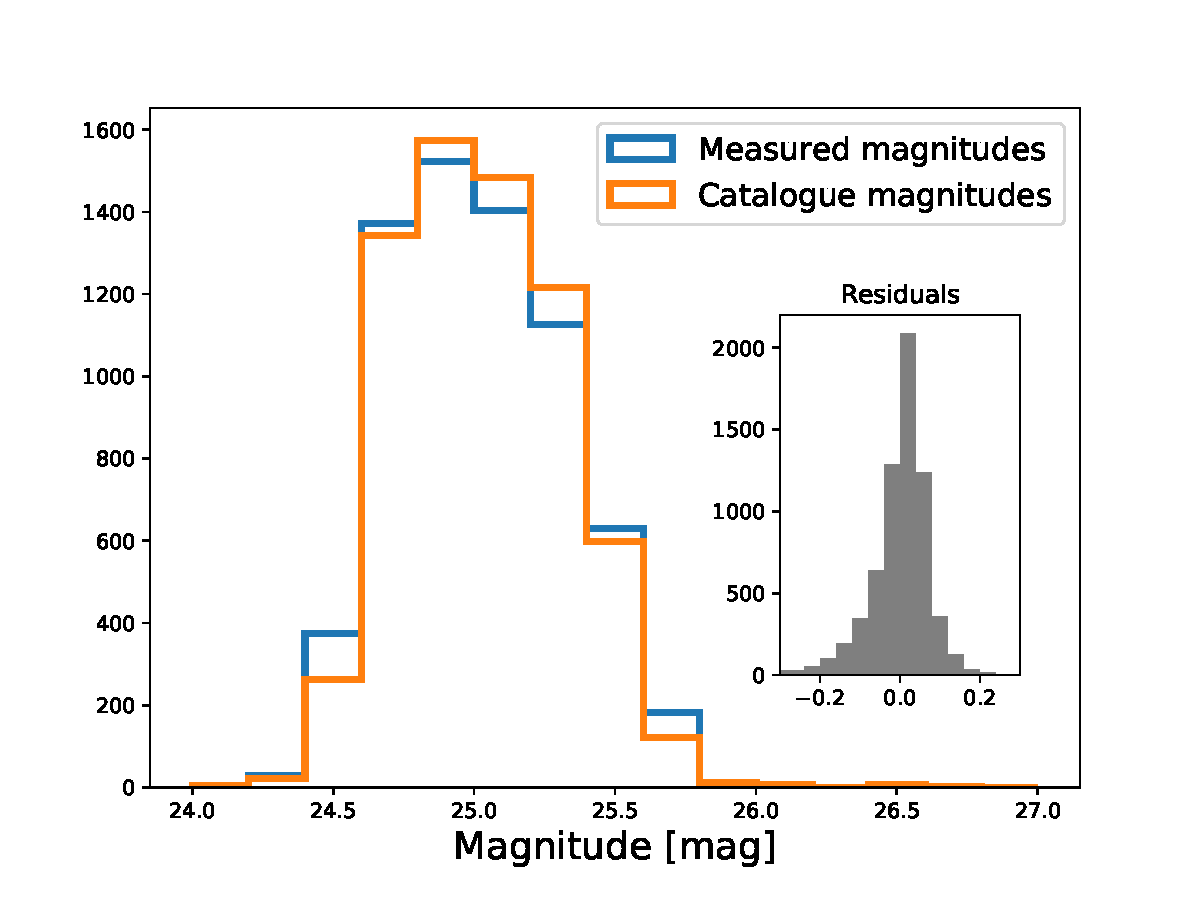
\includegraphics[trim={0.5cm 0 2cm 1.8cm},clip,width=0.45\textwidth]{Code/Saved_Figures/Mag_hist.pdf}
    \caption{The distribution of magnitudes pertaining to objects in the COSMOS field. In blue, the magnitude measurements found by running SEP is plotted. In orange the 2'' magnitudes reported in the COSMOS 2015 catalogue are displayed. In grey a residual plot is shown, mapping the difference between the measured and reported magnitude for each object.}
    \label{mag_hist}  
\end{wrapfigure}

Utilising the software IRACCLEAN presented in \cite{Hsieh_2012_IRACCLEAN}, the sources can be modelled to produce a residual map. The centroids from the SEP algorithm and the total flux found from fixed aperture photometry is used to create point source models of the sources. The point source model is an approximation, since the light profiles of the galaxies might differ from a perfect point source. However, due to the low resolution of the IRAC image, as a result of its peculiarly large point spread function (PSF) that is much bigger than the size of the galaxies modelled, the approximation is deemed reasonable. \textcolor{red}{I should probably make it clear that I didnt actually do this but refer to the author - Iary}. \\ \\
There are, however, limitations to aperture photometry, which is why we explore the possibility of using the COSMOS 2020 FARMER catalogue as a basis for a new residual map of the IRAC image...




\begin{itemize}
    \item SEP to find sources in the telescope img. Briefly mention aperture photometry (which is used in Laigle et al. 2016 -- COSMOS2015) and the fact you did measure aper photometry by yourself as sanity check. However, aper photometry has limitations bla bla bla hence the need for a different approach (Tractor/Farmer)
    \item Describe (very briefly) how the FARMER model parameters are found and adding a reference to Johns paper - something something with many gaussians. 
    \item Describe (again briefly) what the Sersic profile is.
    \item Describe the 5 models we use (exponential, devaucouleur, point source etc.)
    \item Describe the convolution with the psf and why we do it.
    \item Describe how this combined into a residual map, and what we can use it for.
    \item How to create a catalogue containing sources found in the residual map. Matched objects will be included due to imperfections in the residual map, but other more faint objects will also appear. Aperture photometry in original images in different bands provide flux for the object in H, Ks, ch1 and ch2 bands.
\end{itemize}

\subsection{Classification with Semi-supervised ML}
\begin{itemize}
    \item Describe how t-SNE works referring to the original article \cite{Maaten_2008_tSNE} and how it can be used to visualize our data.
    \item Parameter optimization - perplexity = trade of between local and global structures, what is most important here. Visual inspection of options, has to be done for new data. Training and validation data is mapped simulataneously - if new data has to be done again. Description on this is found in \cite{Steinhardt_2020}
    \item Describe our use of tracers that were found by visual inspection. Looking to the detected objects in the different bands we could see if they looked like H-dropout candidates. We assigned good labels to these. \textcolor{red}{Either here or perhaps in the introduction we should describe how we expect the candidates to look like, what features are we looking for when we visually inspect them}
    \item Describe the classification part: K nearest neighbour voting based on the euclidean distance. Elaborate on this choice: we also tried using all neighbours within a radius but due to the t-SNE embedding that essentially projects a higher dimensional manifold into 2d the distances are not necessarily euclidean, different regions has different densities. Varying the fraction of votes "for" to produce ROC curve.
    \item Score metric: ROC curve and AUC, accuracy, and purity/contamination rate.
\end{itemize}